\documentclass{article}
\usepackage[utf8]{inputenc}
\usepackage{graphicx}
	\DeclareGraphicsExtensions{.png, .jpeg}
\usepackage{wrapfig}
\usepackage{caption}
% \usepackage{subcaption}
\usepackage[top=1in, bottom=1in, left=1in, right=1in]{geometry}

\title{Database Design and Implementation \\ HW 01}
\author{\underline{Team 08}\\Henriod, Terence\\Santoyo, Jorge \\Singh, Raja}
\date{\today}

\begin{document}

\maketitle

\begin{abstract}
An introductory/review homework on the topic of databases. Basic relational terminology and Entity Relationship Diagrams (ERDs) using the ``Crow's Foot" notation are explored.
\end{abstract}

\newpage
\begin{enumerate}
	\item Refer to the data model for the Pine Valley Furniture Company in your Modern Database Management text. That data model is Figure 2-22 on on pg. 96 of the 10th edition of the text and pg. 94 of the 11th edition of the text. If you don’t have your book yet, the data model is available on the link “Pine Valley Data Model” in the same cell on the schedule where you found this assignment. Answer the questions below about that data model.
	
  \begin{figure}[h!]
    \centering
    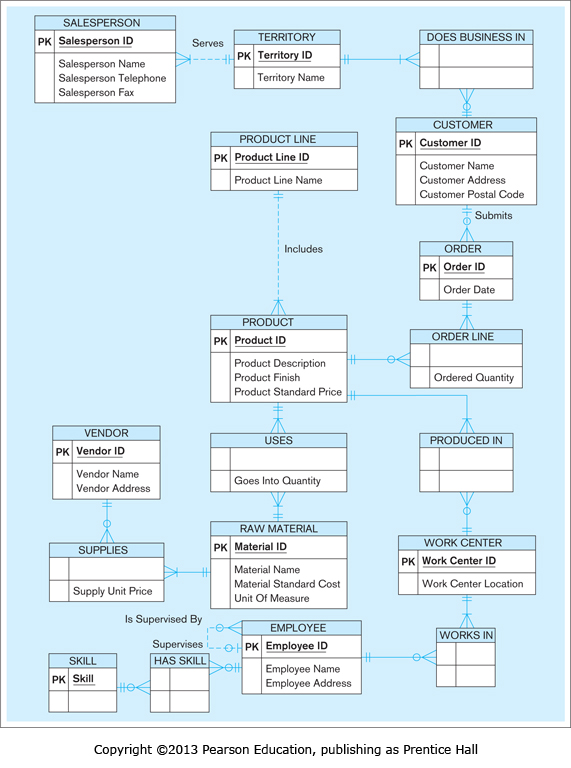
\includegraphics[width=.3\linewidth]{fig02_22}
    \caption{Figure 2-22 from the text.}
    \label{fig:figure_02_22}
  \end{figure}

	\begin{enumerate}
		\item Identify a strong entity on the data model. Provide one reason why you think it is a strong entity.\\

		\textit{Solution}: A CUSTOMER is an example of a strong entity in this context because a CUSTOMER instance can exist on its own; it does not necessarily matter if a customer has made any orders/purchases. Other examples include SALESPERSON and TERRITORY because they can all exist independently of any other entities.\\

		\item Identify a weak entity on the data model. Provide one reason why you think it is a weak entity.\\

		\textit{Solution}: An ORDER LINE is an example of a weak entity in this context because an ORDER LINE instance cannot exist without being part of an order. Further, we could argue that an ORDER is a weak entity because an ORDER cannot be placed without a CUSTOMER to place it.\\

		\item What is the purpose of the WORKS IN entity?\\

		\textit{Solution}: WORKS IN is an Associative (or Intersection) Entity. It's purpose is to help store data that would not belong in either EMPLOYEE or WORK CENTER but that is specific to an employee-work center relationship instance, such as what responsibilities a certain employee has at a specific work center, for example.\\

		\item The WORKS IN entity has two binary relationships – one with the WORK CENTER entity and one with the EMPLOYEE entity. Look at the cardinalities of those two relationships and explain in words the meaning of those two binary relationships.\\

		\textit{Solution}:
			\begin{description}
				\item[WORKS IN and WORK CENTER] Each WORKS IN instance has exactly one WORK CENTER instance it is related to, while a WORK CENTER instance can be related to many WORKS IN instances. In other words, a WORK CENTER will require data about the 1 to many employees that work there (there must be at least one because it can't be a place of work if no one works there), but each WORKS IN instance can only describe work at one location.\\

				\item[WORKS IN and EMPLOYEE] An EMPLOYEE could work in any number of work centers, thus needing any number of WORKS IN instances (maybe they are no longer employed, they work at one location exclusively, or they visit multiple locations); a WORKS IN instance can reference one and only one EMPLOYEE instance because it would describe the employee's work at one particular work location.\\
			\end{description}

		\item What would be an appropriate primary key for the WORKS IN entity? Explain why you chose that primary key for the WORKS IN entity.\\

		\textit{Solution}: A concatenated key of the Work Center ID from WORK CENTER and the Employee ID from EMPLOYEE should suffice to uniquely identify a WORKS IN instance.\\

		\item The WORKS IN entity has no attributes on the data model. Name at least one non-key attribute that you believe might be stored in that entity.\\

		\textit{Solution}: The number of hours, percentage of work time, or frequency that an employee works at a particular location would be a good candidate attribute for the WORKS IN entity.\\

		\item Make up three sample rows of data each for the WORK CENTER, EMPLOYEE and WORKS IN entities. If you don’t understand what I mean by “sample data,” refer to the first week exercise, questions 8, 9, 10 that we completed in class. If you weren’t in class, then look at figure 1-16 of your text.\\
		
  \textit{Solution}:
  \begin{figure}[h]
    \centering
    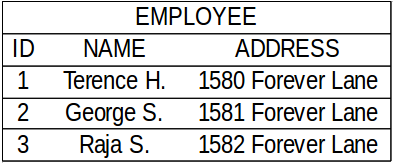
\includegraphics[width=.2\linewidth]{HW01_Part01_g1}
    \caption{EMPLOYEE sample data.}
    \label{fig:employee_sample}
  \end{figure}

  \begin{figure}[h]
    \centering
    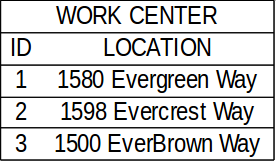
\includegraphics[width=.15\linewidth]{HW01_Part01_g2}
    \caption{WORK CENTER sample data.}
    \label{fig:work_center_sample}
  \end{figure}
  
  \begin{figure}[h]
    \centering
    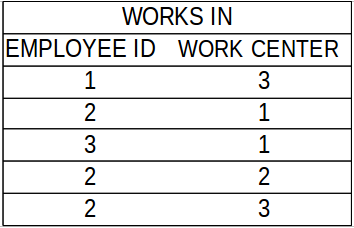
\includegraphics[width=.2\linewidth]{HW01_Part01_g3}
    \caption{WORKS IN sample data.}
    \label{fig:works_in_sample}
  \end{figure}

	\end{enumerate}

	\newpage
	\item Use the business rules below to identify and write all attributes, relationships and cardinalities between the entities shown on the next page. Decide which attributes should be primary keys and foreign keys for each entity and put those in the diagram. Remember to include relationship verbs for all relationships. The application is for a charter airline company that flies planes for clients. The database will be owned by the charter airline company. There are no regularly scheduled flights; all flights occur when a charter client schedules and purchases a given flight. If you need to make assumptions about business rules other than the ones provided below, be sure to write those assumptions on your answer.\\

	\begin{itemize}
		\item An aircraft is uniquely identified by an AircraftID. For each aircraft, the database should keep track of the type of plane it is and the quantity of seats.\\
		\item A client is uniquely identified by a ClientID. For each client, the database should keep track of the client name and phone number.\\
		\item A pilot is uniquely identified by a PilotID. The database should keep track of the name and phone number for each pilot.\\
		\item One instance of a flight is assigned to only one aircraft, one pilot and one client. An aircraft could potentially be used on multiple flights. A client could potentially contract with the charter airline company for multiple flights.\\
		\item For each flight, the charter airline company wants to store the start date and time of the flight, the aircraftID for the flight, the pilotID, and the clientID for the flight. You need to determine which attribute(s) should compose the primary key for the flight entity.\\
	\end{itemize}

	\textit{Solution}:\\
	\begin{figure}[h!]
    \centering
    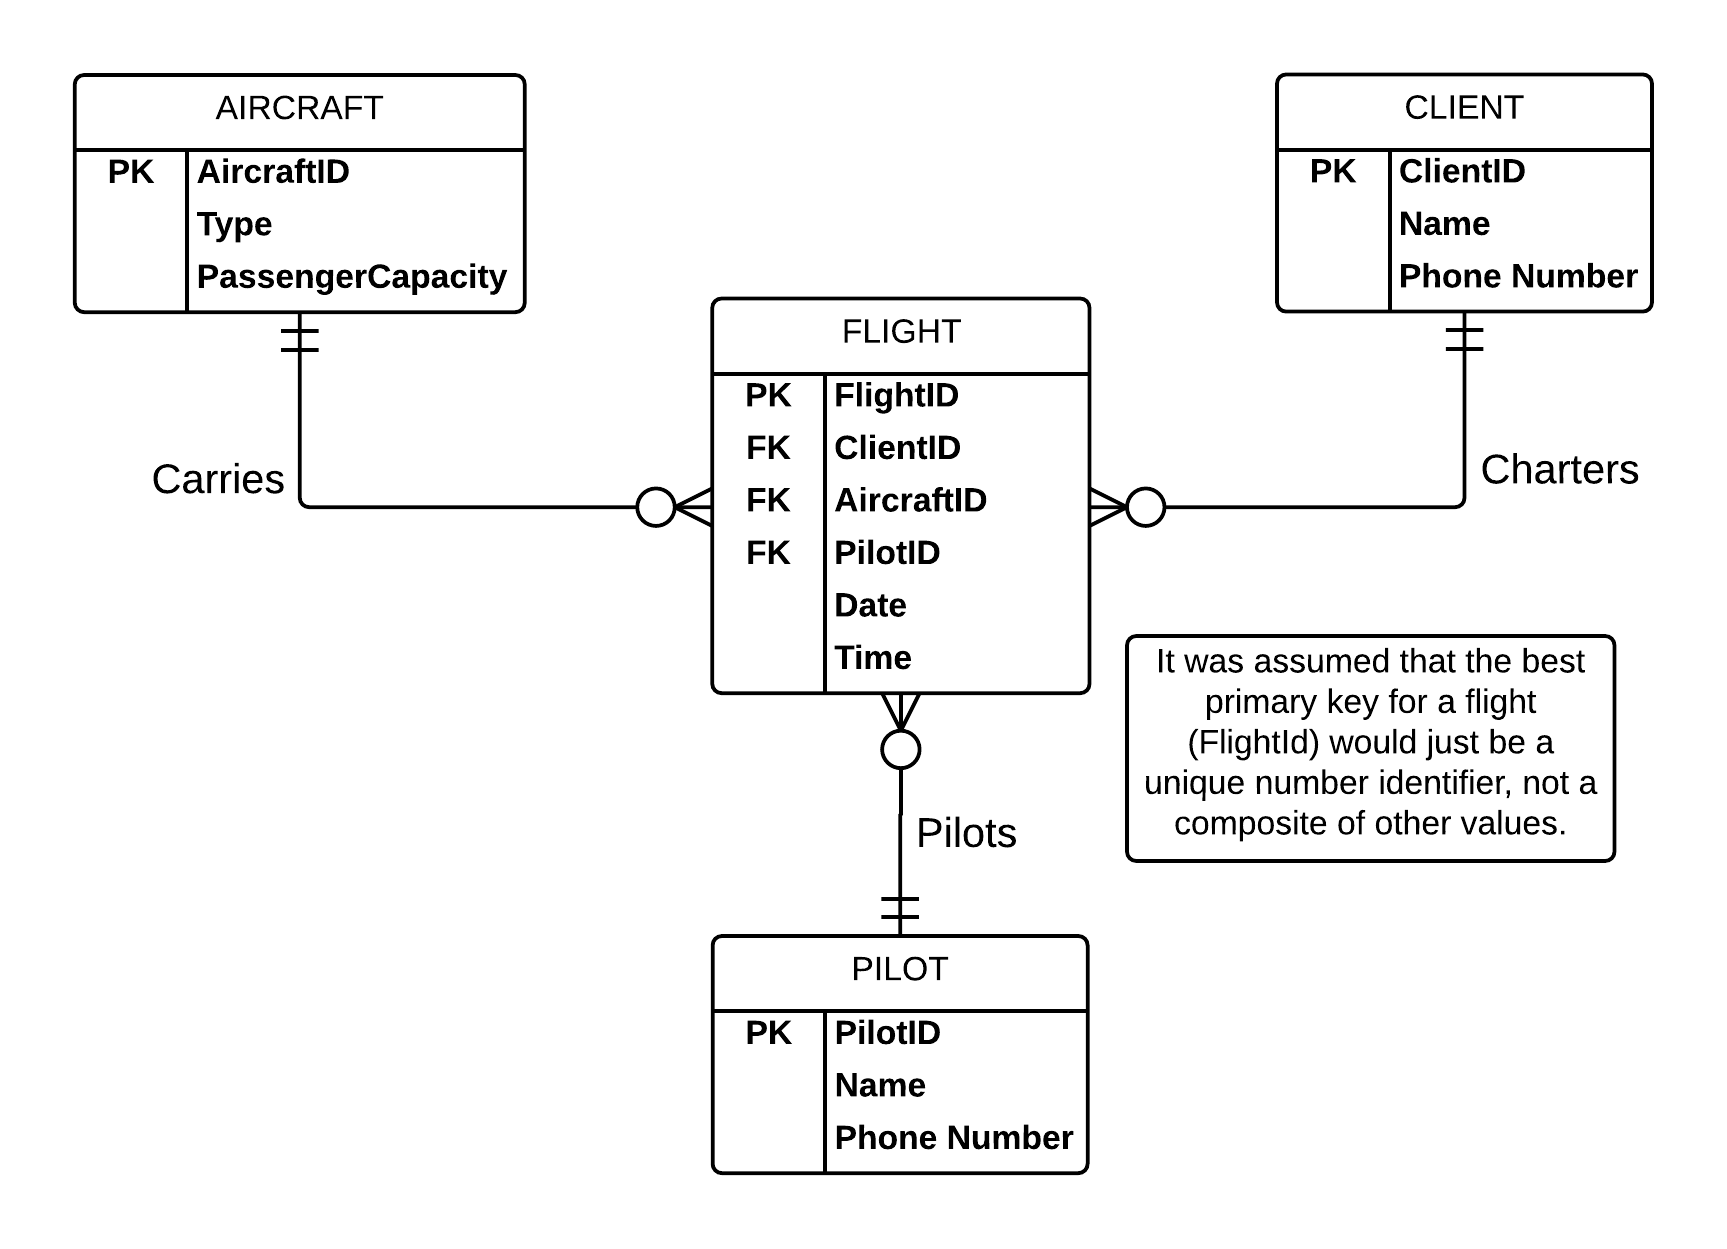
\includegraphics[width=.7\linewidth]{HW01_Part02-ERD}
    \caption{The ERD for the charter airline company's database (Problem 2).}
    \label{fig:part_02_erd}
  \end{figure}

	\newpage
	\item Create a logical ERD for each of the problems below using the crowsfoot notation discussed in class. Be sure that each entity is a box with the name of the entity at the top of the box, the primary key attribute or attributes in the middle of the box, and the non-primary key attributes in the bottom of the box. Lines should separate each part of the entity box. Each entity must have a primary key defined. A primary key may consist of one of more attributes. \\
	The final ERD submitted for grading should not include any M:N relationships and all attributes should be placed within an entity. Each relationship should have at least one relationship verb or verb phrase. Please include all required foreign keys and denote the foreign key(s) with the notation (FK) on the ERD. \\
	Do not use Visio for this assignment, but please make sure the ERDs are readable. I recommend using a ruler/straight-edge for the entities and relationships. For the first problem – problem (a) - I provide some sample data to help you understand the type of data that would be stored in the database. I recommend that you do the same thing for the other two problems. It is always easier to figure out how you are going to store the data once you know what types of data will be stored. You do not have to turn in sample data – the only required deliverable is one ERD per problem.\\

	\textit{We did not use Visio to create our ERDs - we used a software called Lucidchart. We hope that this was not against any rules, but our need for high productivity mixed with a little OCD led us to use a software that we were already familiar with to produce a clean product.}\\

	\newpage
	\begin{enumerate}
		\item A college course is taught by many instructors, and an instructor may teach many courses. An instructor teaches a section of a course. A course may have one or more scheduled sections, or may not have a scheduled section. Attributes of COURSE include courseID, coursename, and credits. A courseID is a unique value for a given course. Attributes of a SECTION of a course include courseID, sectionID, semesternumber, year, and instructorID. A given section of a course is taught by only one instructor. An INSTRUCTOR is identified by an instructorID. Additional information we want to store about an instructor includes the lastname, firstname, and officenumber. We want to store the quantity of students registered for a course. Sample data for this application system is provided below.\\

  \begin{figure}[h!]
    \centering
    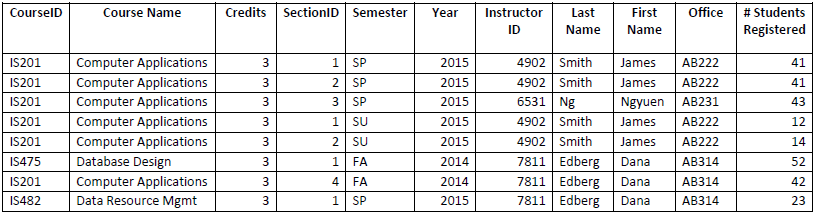
\includegraphics[width=.7\linewidth]{HW01_Part03_TableA}
    \caption{Sample data for problem 3-a.}
    \label{fig:03_a_sample_data}
  \end{figure}
  
  \textit{Solution}:
  \begin{figure}[h!]
    \centering
    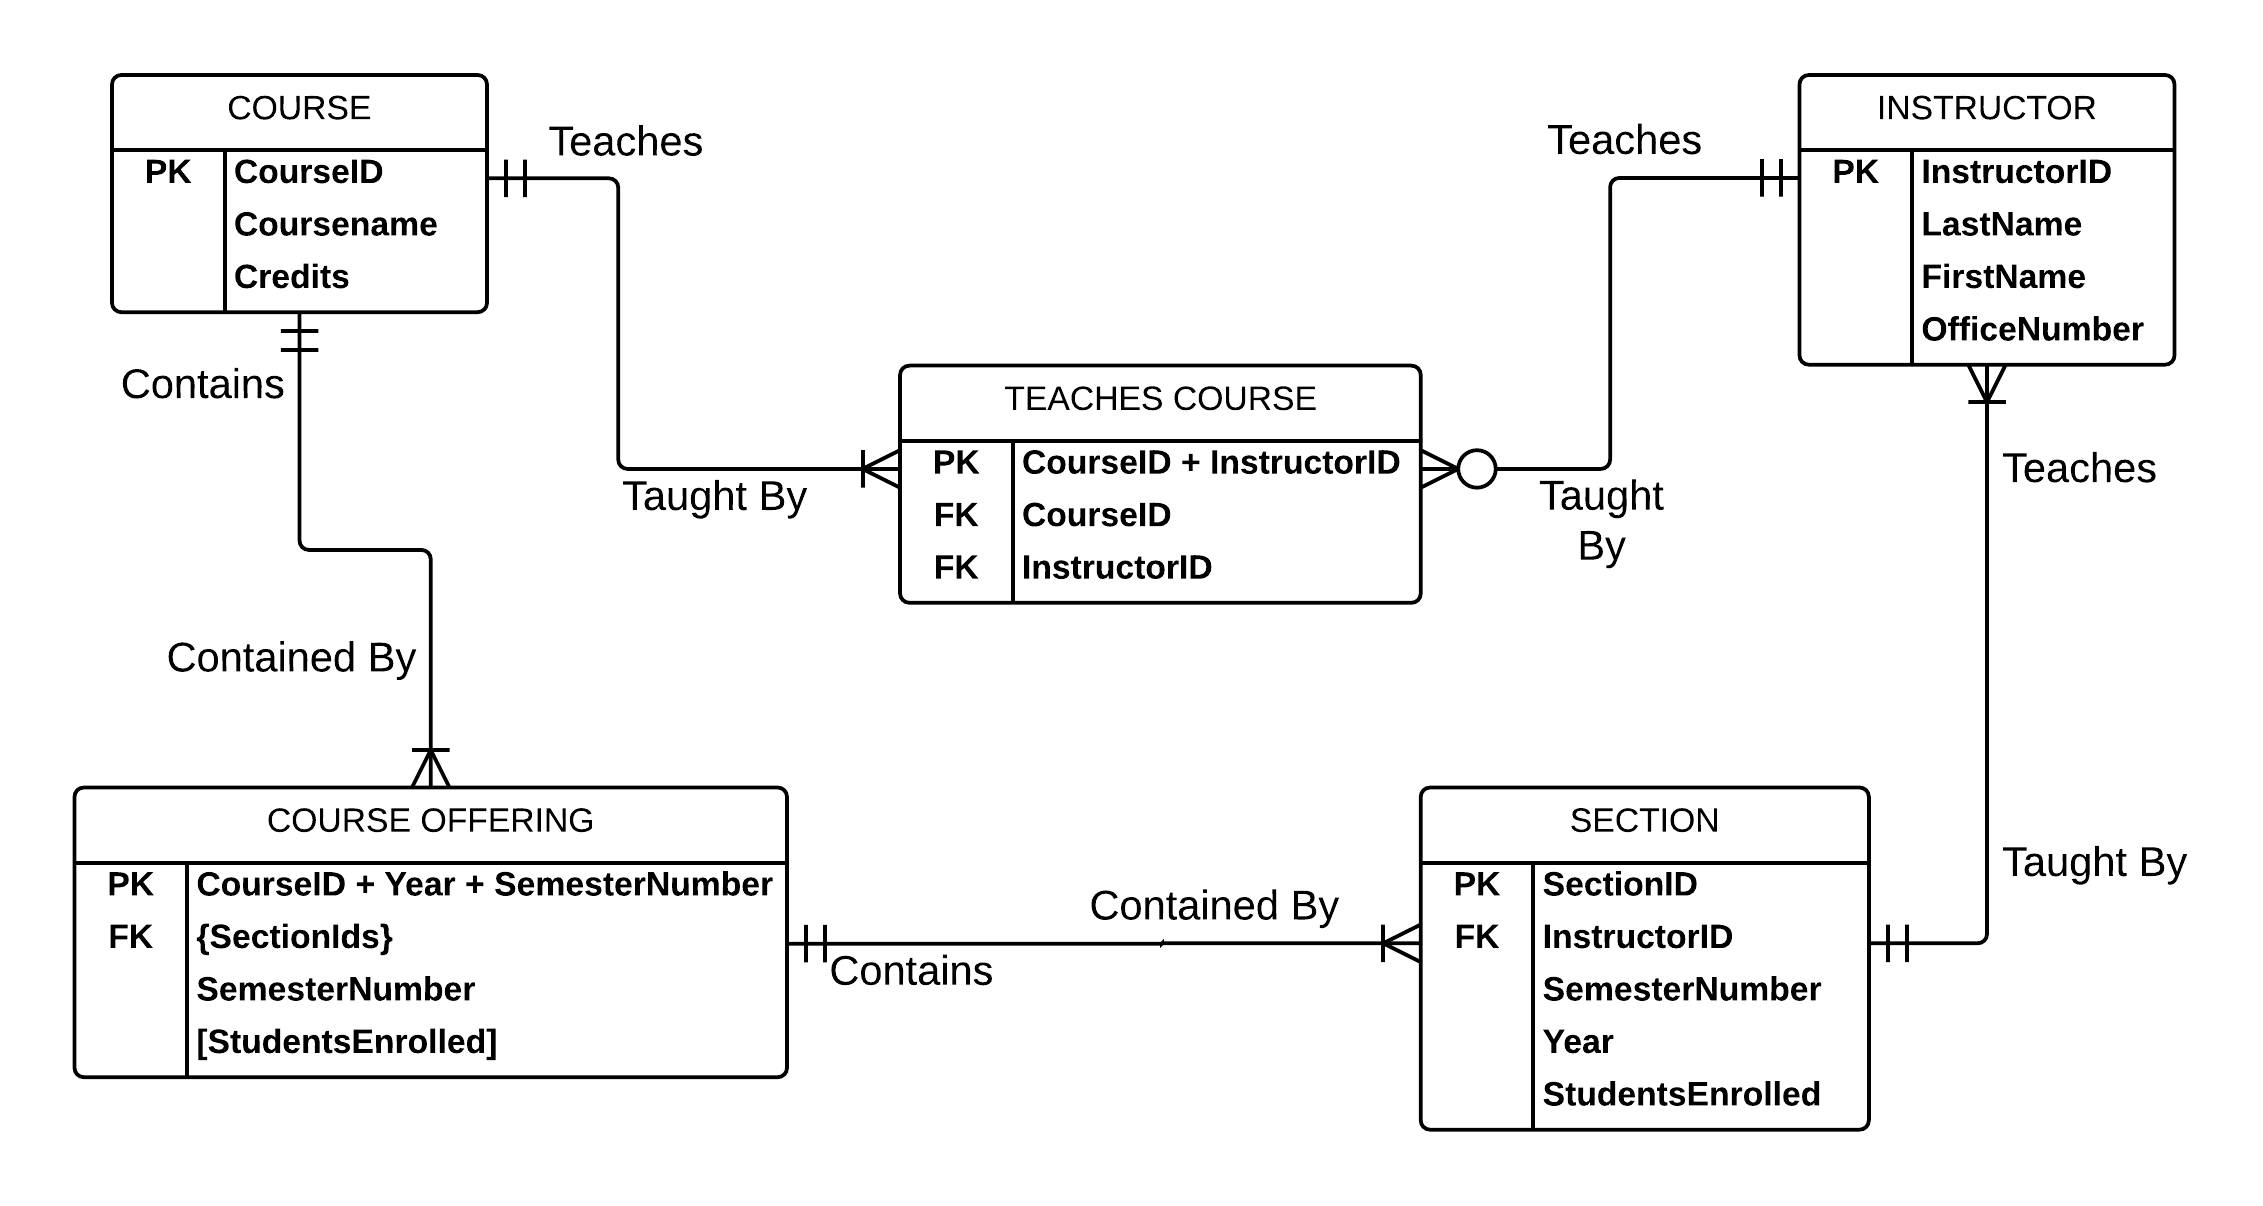
\includegraphics[width=.8\linewidth]{HW01_Part03_a-ERD}
    \caption{The logical ERD for the college (Problem 3-a).}
    \label{fig:03_a_solution}
  \end{figure}

		\newpage
		\item A corporation owns a series of shopping malls. A shopping mall has one or more stores; a shopping mall isn’t a shopping mall unless there is at least one store at the mall. Each shopping mall has similar stores (examples are: Footlocker, Walking Company, Jones New York, Abercrombie and Fitch) but each store is physically different at each mall. Each shopping mall is identified by a MallID. For each shopping mall, we want to keep track of the name of the mall, the address, zip code, and main telephone number. A shopping mall can have multiple stores, a store can be in multiple shopping malls. Each store is identified by a StoreID. For each store, we want to keep track of the name of the store and a long description of the type of the store. The corporation needs to associate a specific instance of a store with a shopping mall. For a specific instance of a store at a given shopping mall, the corporation wants to keep track of the date the store opened at the mall, the name of the manager for the store, and the telephone number for that specific instance of a store in that mall. If you were viewing the data for this application in a spreadsheet format, it would look like the data shown below:\\

% there's a table that goes here
  \begin{figure}[h!]
    \centering
    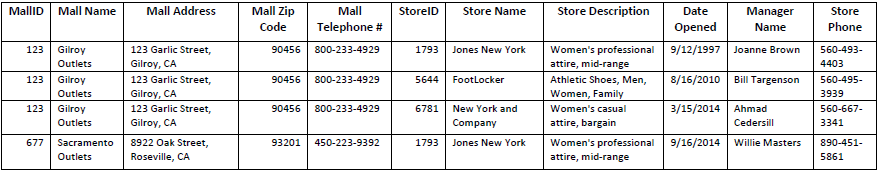
\includegraphics[width=.7\linewidth]{HW01_Part03_TableB}
    \caption{Sample data for problem 3-b.}
    \label{fig:03_b_sample_data}
  \end{figure}
  
  \textit{Solution}:
  \begin{figure}[h!]
    \centering
    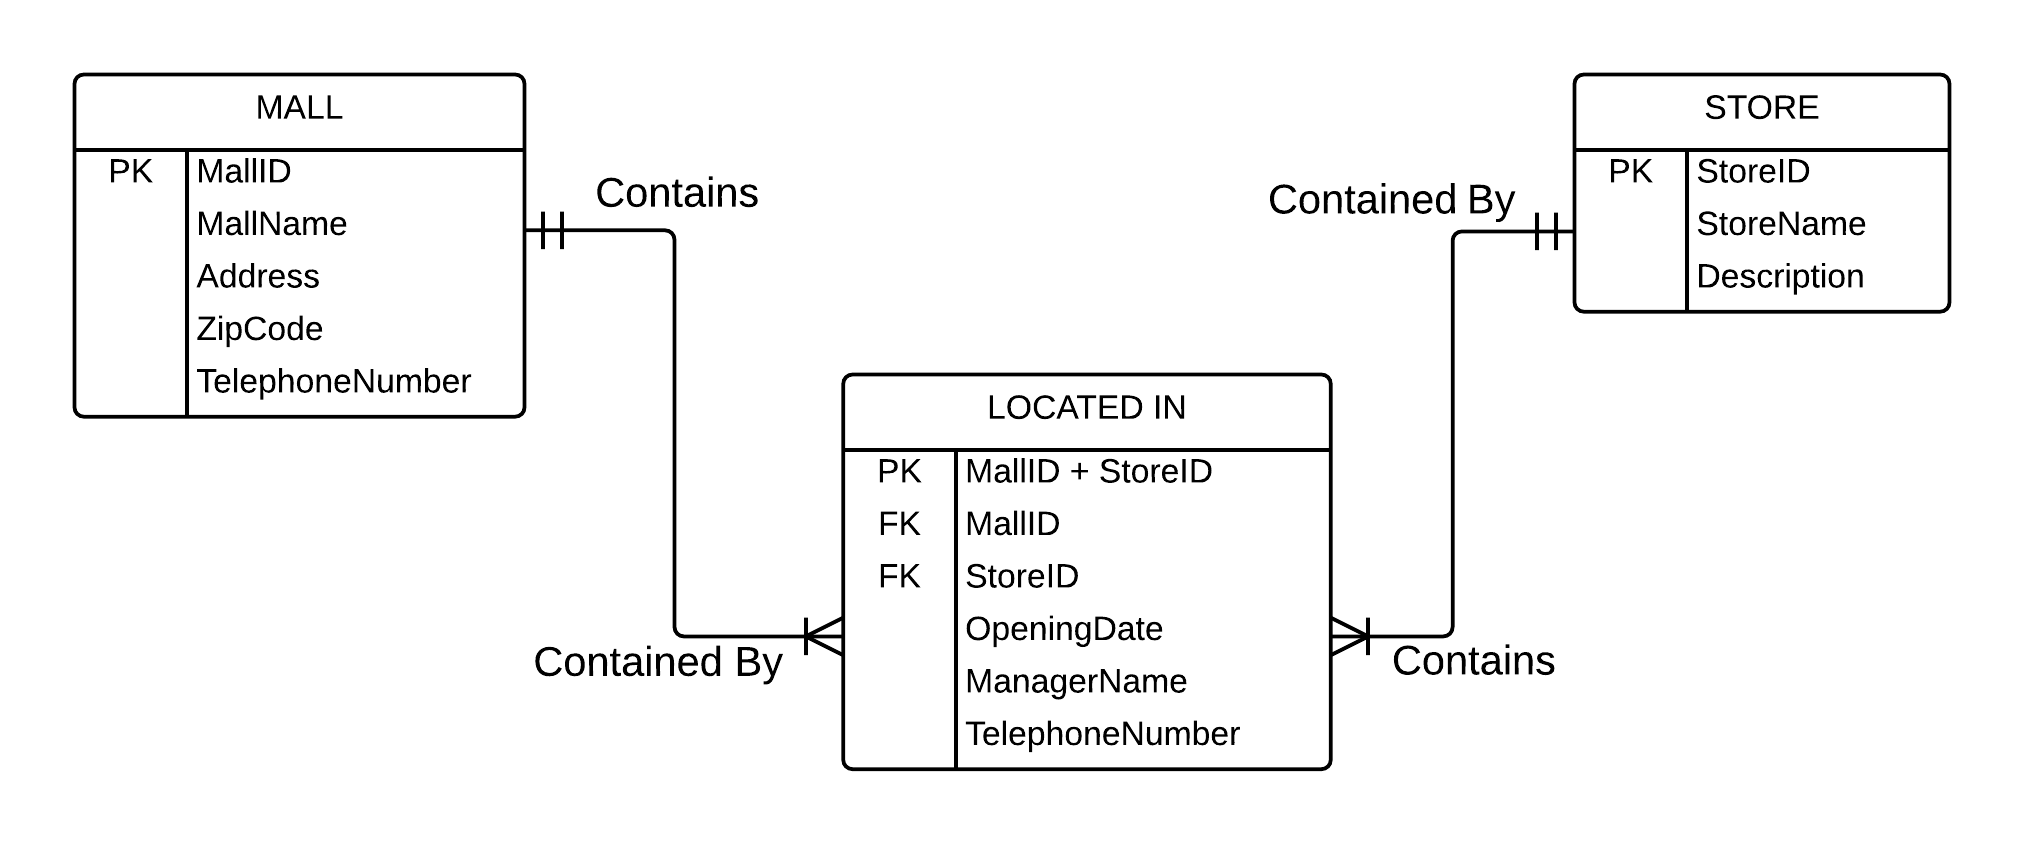
\includegraphics[width=.8\linewidth]{HW01_Part03_b-ERD}
    \caption{The logical ERD for the mall corporation (Problem 3-b).}
    \label{fig:03_b_solution}
  \end{figure}
	\end{enumerate}

\end{enumerate}

\end{document}
